\section{Data set and time definition}\label{sec:data_time}

In Sect. \ref{subsec:data_set} we introduce the data set used in the paper. In
Sect. \ref{subsec:physical_time} we describe the physical time scale and in
Sect. \ref{subsec:trade_time} we describe the trade time scale.

\subsection{Data set}\label{subsec:data_set}

In this study, we have analyzed trades and quotes (TAQ) data from the NASDAQ
Stock Market. We selected NASDAQ because it is an electronic exchange where
stocks are traded through an automated network of computers instead of a
trading floor, which makes trading more efficient, fast and accurate.
NASDAQ is the second largest stock exchange based on market capitalization in
the world.

In the TAQ data set, there are two data files for each stock. One gives the
list of all successive quotes. Thus, we have the best bid price, best ask price,
available volume and the time stamp accurate to the second. The other data file
is the list of all successive trades, with the traded price, traded volume and
time stamp accurate to the second. Despite the one second accuracy of the time
stamps, in both files more than one quote or trade may be recorded in the same
second.

Due to the the time stamp accuracy, it is not possible to match each trade with
the directly preceding quote. Hence, we cannot determine the trade sign by
comparing the traded price and the preceding midpoint price
\cite{Wang_2016_cross}. In this case we need to do a preprocessing of the data
to relate the midpoint prices with the trade signs in trade time scale and in
physical time scale. Observe that we will not be discussing the returns, but
the midpoint price. This because both are intrinsically related, as explained
before, and it is more intuitive to understand the changes in midpoint prices
than in returns.

To analyze the response functions across different liquid stocks, we select the
six companies with the largest average market capitalization (AMC) (Alphabet
Inc., Mastercard Inc., CME Group Inc., Goldman Sachs Group Inc., Transocean
Ltd. and Apache Corp.) in three economic sectors (information technology,
financials and energy) of the S\&P index in 2008.

In order to avoid overnight effects and any artifact due to the opening and
closing of the market, we systematically discarded the first ten and the last
ten minutes of trading in a given day
\cite{spread_changes_affect,Bouchaud_2004,Wang_2016_cross,large_prices_changes}.
Therefore, we only consider trades of the same day from 9:40:00 to 15:50:00
New York local time.

\subsection{Trade time scale}\label{subsec:trade_time}

We use the trade sign classification in trade time scale proposed by S. Wang et
al. in \cite{Wang_2016_cross} and used in
\cite{Wang_2016_avg,Wang_2017,Wang_2018_copulas} that reads

\begin{equation}\label{eq:trade_signs_trade}
    \varepsilon^{trade}\left(t,n\right)=\left\{
    \begin{array}{cc}
    \text{sgn}\left(S\left(t,n\right)-S\left(t,n-1\right)\right),
    & \text{if }\\ S\left(t,n\right) \ne S\left(t,n-1\right)\\
    \varepsilon\left(t,n-1\right),
    & \text{otherwise}
    \end{array}\right.
\end{equation}

With this classification we obtain trade signs for every single trade in the
data set. According to \cite{Wang_2016_cross}, the average accuracy of the
classification is $85\%$ for the trade time scale.

For the trade time scale, as the TAQ time step is one second, and as it is
impossible to find the correspondences between trades and midpoint prices
values inside a second step, We used the last midpoint price of every second as
the representative value of each second. This introduce an apparent shift
between trade signs and returns. In fact, we set the last midpoint price from
the previous second as the first midpoint price of the current second, as
explained in \cite{Wang_2016_cross}.

As we know the second in which the trades were made, we can relate the trade
signs and the midpoint prices as shown in Fig.
\ref{fig:relation_trades_midpoint_trade_scale}. For the trade time scale, they
are in some cases, several midpoint prices in a second. For each second we
select the last midpoint price value, and we relate it to the next second
trades. In Fig. \ref{fig:relation_trades_midpoint_trade_scale}, the last
midpoint price between the second $-1$ and $0$ is related with all the trades
in the second $0$ to $1$, and so on. In the seconds that there is no change in
the quotes, it is used the value of the previous second. In consequence, all
the seconds in the open market time have a midpoint price value.

\begin{figure}[htbp]
    \centering
    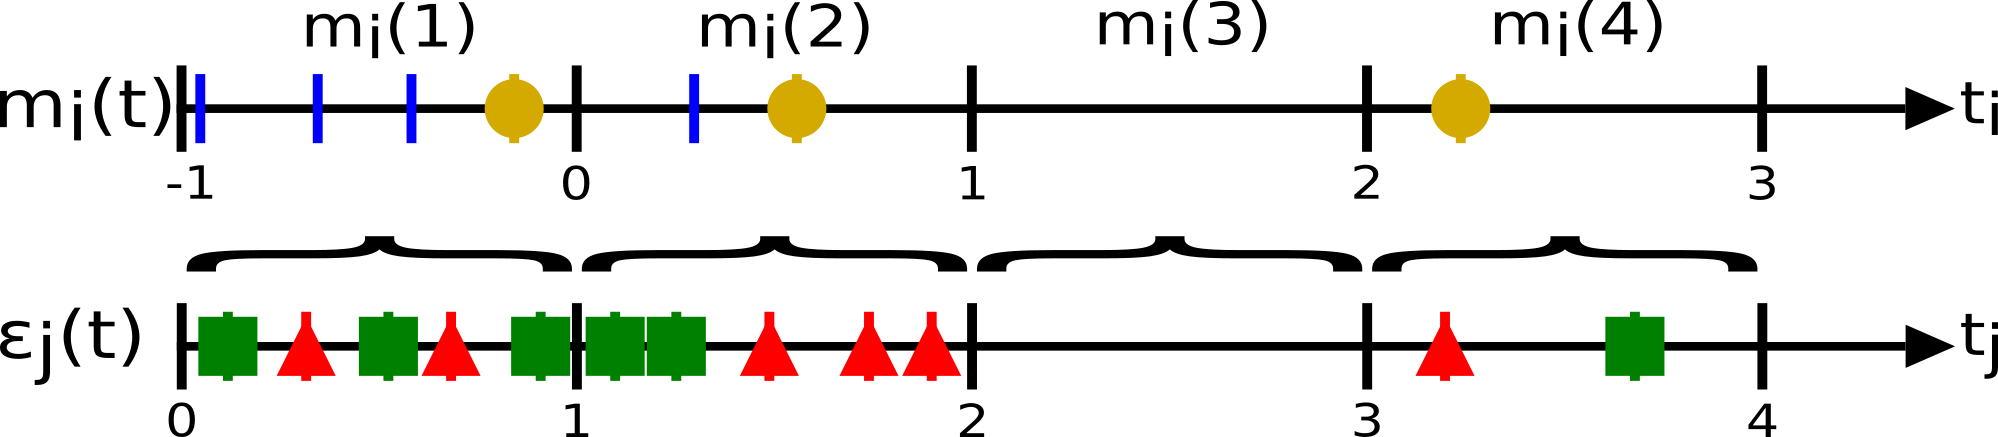
\includegraphics[width=\columnwidth]{figures/02_relation_trades_quotes_trade_scale.png}
    \caption{Sketch of data processing for trade time scale. Each trade sign is
             related with the last value of the midpoint price of the previous
             second.}
    \label{fig:relation_trades_midpoint_trade_scale}
\end{figure}

We computed all the analysis for the trade time scale using Equations
\ref{eq:midpoint_price_return} and \ref{eq:trade_signs_trade}.

The methodology described is an approximation to compute the response in the
trade time scale. A drawback in the computation could come from the fact that
the return of a given second is composed by the contribution of small returns
corresponding to each change in the midpoint price during a second. As we are
assuming only one value for the returns in each second, we are supposing  all
the returns in one second interval to be positive or negative, which could not
be the case. This could increase or decrease the response signal at the end of
the computation.

\begin{figure}[htbp]
    \centering
    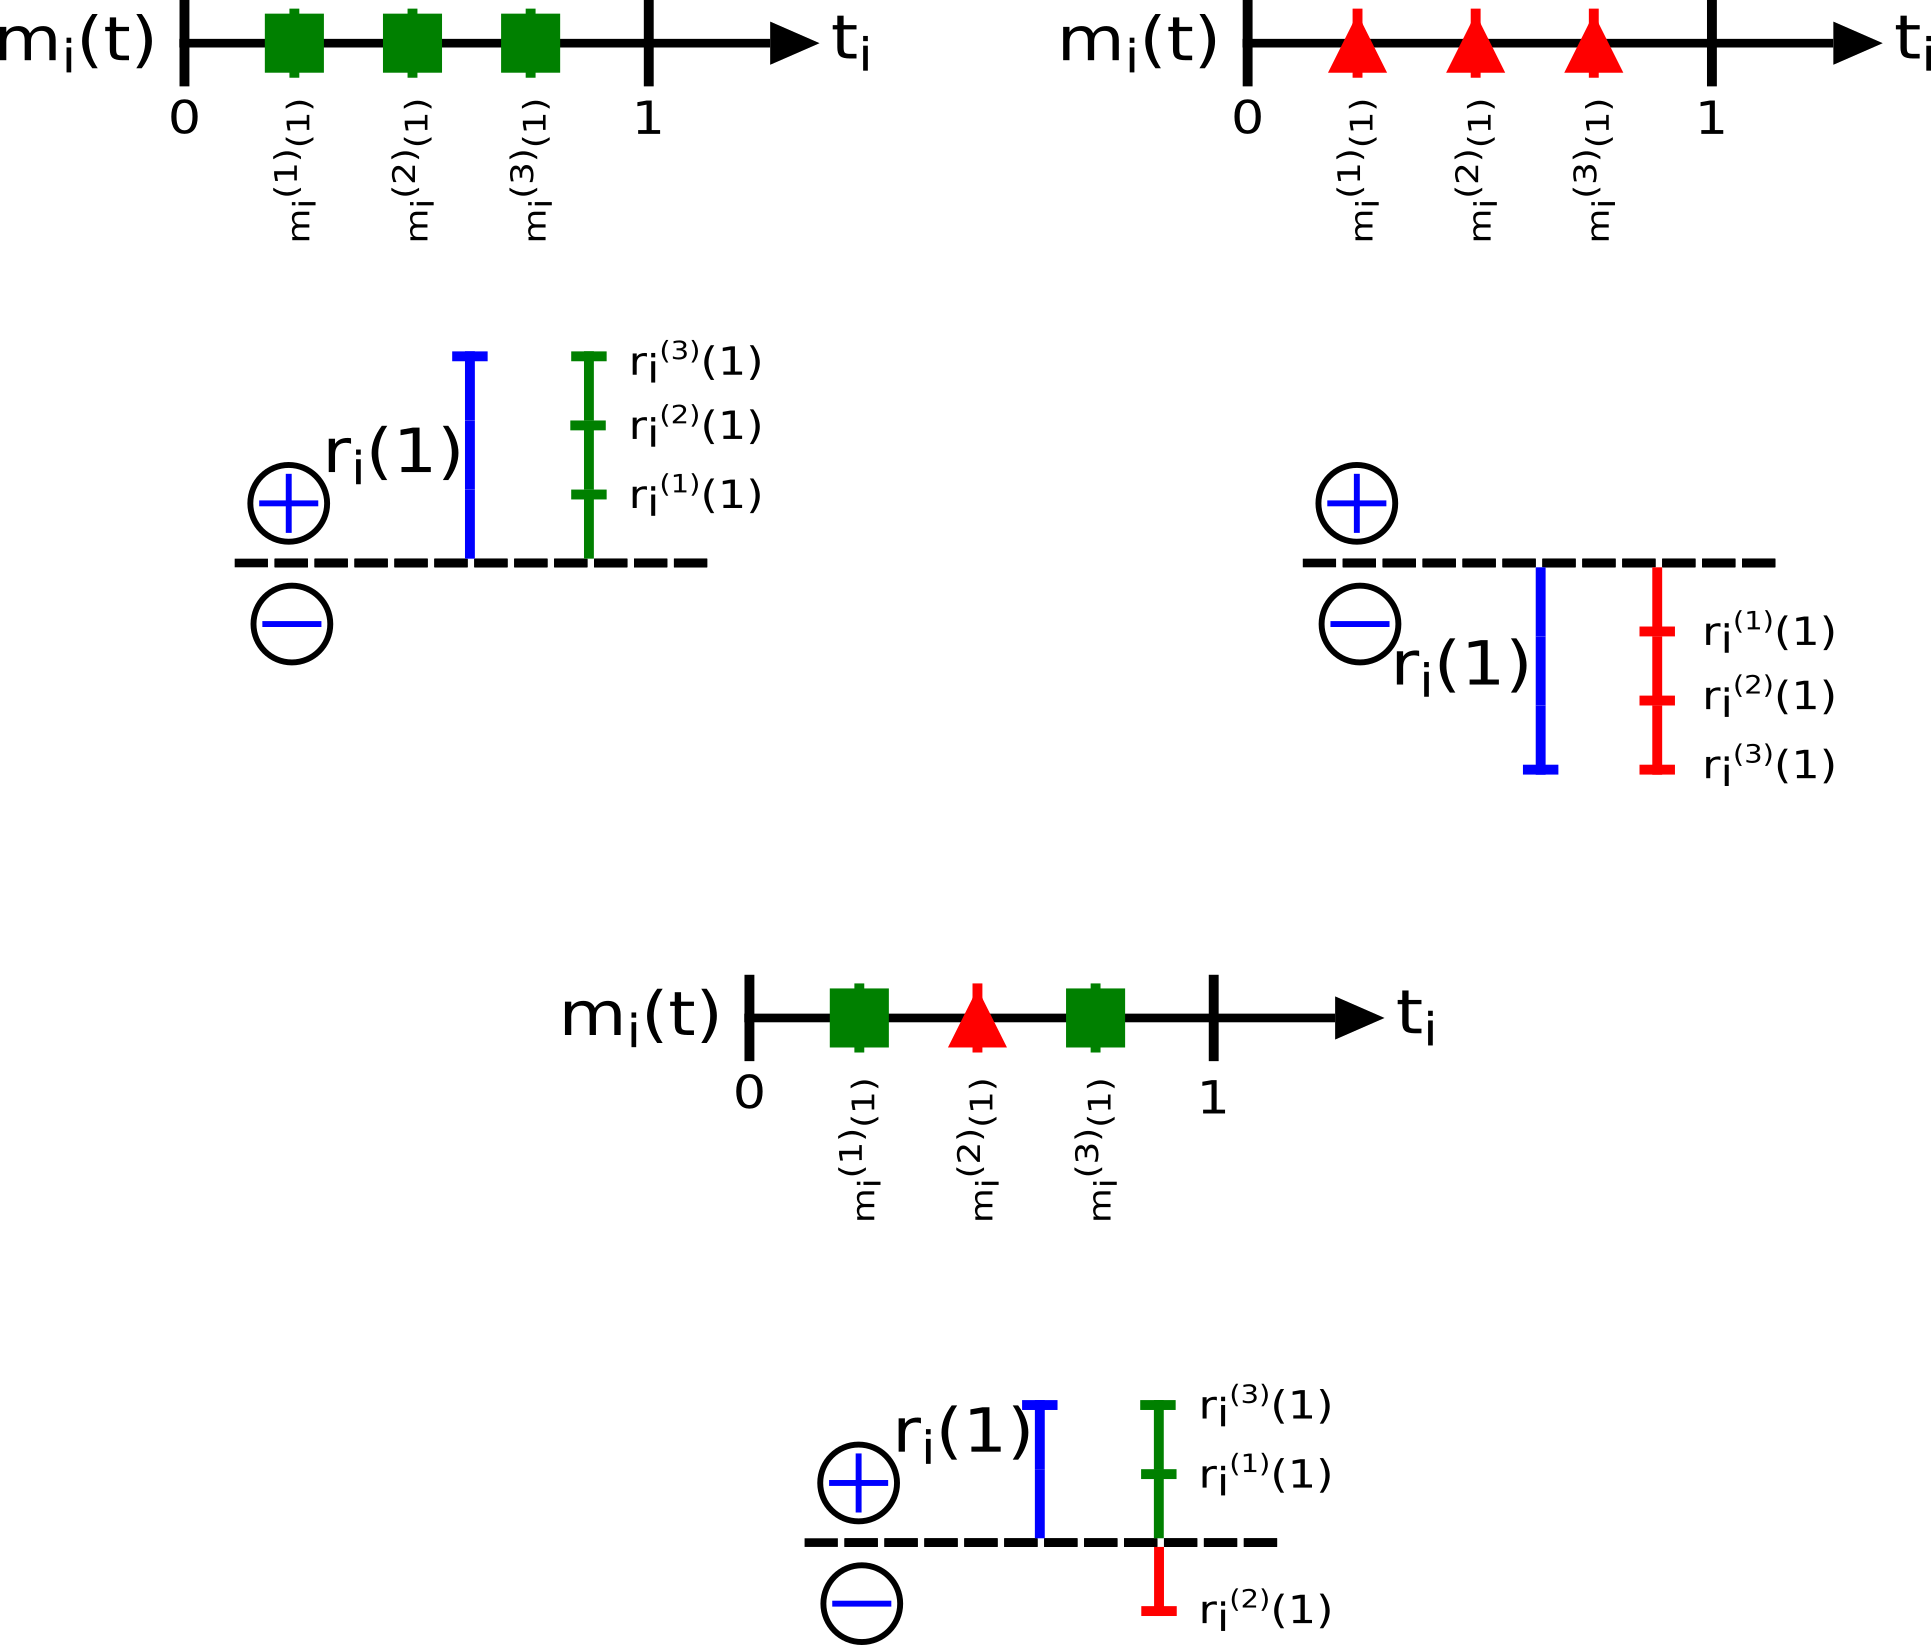
\includegraphics[width=\columnwidth]{figures/02_return_contributions.png}
    \caption{Sketch of the return contributions from every midpoint price
             change in a second. We illustrate three cases: (left) the changes
             of the returns and midpoint price are due to buys, (center) the
             changes of the returns and midpoint prices are due to sells, and
             (right) the changes of the returns and midpoint prices are due to
             a combination of buys and sells.}
    \label{fig:return_contributions}
\end{figure}

Figure \ref{fig:return_contributions} illustrate with one example this point.
Suppose one second interval, in which they are three different midpoint prices,
and in consequence, three different returns. Furthermore, consider that the
volume of limit orders that have the corresponding midpoint price are the same
in the bid and in the ask (so the impact have the same magnitude). In the case
of the left (center), all the changes are due to buys (sells), that means,
consumption of the best ask (bid), so all the contributions of the individual
returns in the second are positive (negative), and in consequence, the return
is positive (negative). Finally, in the case of the right, the changes are due
to a combination of buys and sells, so in the end the individual returns sum up
to a net return, which can be positive or negative, depending of the type of
midpoint price in the interval. Thus in this case, we are assuming at the end
that all the returns were positive or negative, what probably was not the case,
and in consequence will increase or decrease the real return.

In all the cases we choose the last change in the midpoint price in a second
interval as described before
(Fig. \ref{fig:relation_trades_midpoint_trade_scale}). We use this method
knowing that the variation in one second of the midpoint price is not large, so
it can give us valuable information about the responses.

\textcolor{red}{Por hacer: - Revisar en promedio cuantos midpoint price por
                segundo en los datos TAQ, - Hallar el porcentaje de cuanto
                cambia el valor del último midpoint price en un segundo con
                respecto al promedio de ese segundo}

\subsection{Physical time scale}\label{subsec:physical_time}

We use the trade sign definition in physical time scale proposed by
S. Wang et al. in \cite{Wang_2016_cross} and used in
\cite{Wang_2016_avg,Wang_2017}, that depends on the classification in
Eq. \ref{eq:trade_signs_trade} and reads

\begin{equation}\label{eq:trade_signs_physical}
    \varepsilon^{physical}\left(t\right)=\left\{
    \begin{array}{cc}
    \text{sgn}\left(\sum_{n=1}^{N\left(t\right)}\varepsilon^{trade}
    \left(t,n\right)\right),
    & \text{If }N \left(t\right)>0\\
    0, & \text{If }N\left(t\right)=0
    \end{array}\right.
\end{equation}

Where $N \left(t \right)$ is the number of trades in a second interval. For
this classification, they are two ways to obtain
$\varepsilon^{physical}\left( t \right) = 0$. The first way is that in a
particular second there is not trades, and then no trade sign. The second  way
is that the addition of the trade signs ($+1$ and $-1$) be equal to zero. In
this case, could be important to see how is the distribution of the trade scale
trades signs for the particular second.

\begin{figure}[htbp]
    \centering
    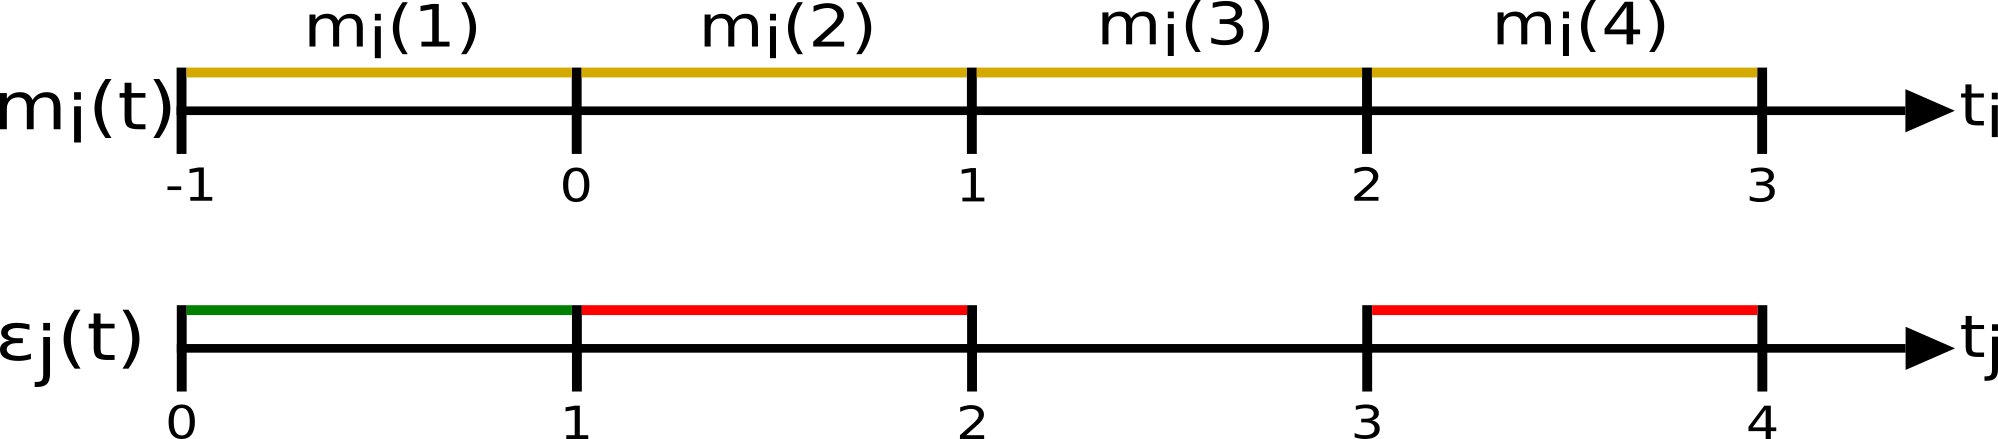
\includegraphics[width=\columnwidth]{figures/02_relation_trades_quotes_time_scale.png}
    \caption{Sketch of data processing for trade time scale. Each trade sign is
             related with the last value of the midpoint price of the previous
             second.}
    \label{fig:relation_trades_midpoint_time_scale}
\end{figure}

$\varepsilon^{physicals}\left( t \right) = +1$ implies that the majority of
trades in second $t$ were triggered by a market order to buy, and a value
$\varepsilon^{physicals}\left( t \right) = -1$ indicates a majority of sell
market orders.

Market orders show opposite trade directions to limit order executed
simultaneously. An executed sell limit order corresponds to a buyer-initiated
market order. An executed buy limit order corresponds to a seller-initiated
market order.

As in the trade time scale, in the physical time scale I use the same strategy
to obtain the midpoint price for every second, so all the seconds in the open
market time have a midpoint price value.

In this case we do not compare every single trade, but the trade obtained for
every second with the classification. This can be seen in
Fig. \ref{fig:relation_trades_midpoint_time_scale}, we relate the midpoint
price of the previous second with the trade sign of the current second.

According to \cite{Wang_2016_cross}, this classification has an average
accuracy up to $82\%$ in the physical time scale.